\begin{frame}{Features}
    \begin{columns}
        \begin{column}{0.5\textwidth}
            \resizebox{\linewidth}{!}{
            \begin{tabular}{|l|l|}
                \hline
                eta\_jf          & forward jet eta                        \\ \hline
                pt\_jf           & forward jet transverse momentum        \\ \hline
                mass\_jf         & forward jet mass                       \\ \hline
                phi\_jf          & forward jet phi                        \\ \hline
                eta\_b           & b-jet eta                              \\ \hline
                pt\_b            & b-jet transverse momentum              \\ \hline
                phi\_b           & b-jet phi                              \\ \hline
                HvisMass         & mass of LorentzV sum of hadronic taus  \\ \hline
                m\_met           & Missing energy                         \\ \hline
                Reco\_w\_mass\_2 & Reconstructed mass of the W case 1     \\ \hline
                Reco\_w\_mass\_1 & Reconstructed mass of the W case 2     \\ \hline
            \end{tabular}}
        \end{column}
        \begin{column}{0.5\textwidth}
            \resizebox{\linewidth}{!}{
            \begin{tabular}{|l|l|}
                 \hline
                 deltaRTau        & Delta R of the hadronic taus          \\ \hline
                 deltaPhiTau      & Delta phi of the hadronic taus        \\ \hline
                 HvisPt           & of LorentzV sum of hadronic taus      \\ \hline
                 HvisEta          & of LorentzV sum of hadronic taus      \\ \hline
                 TvisMass         & mass of reconstructed top             \\ \hline
                 TvisPt           & pt of visible top                     \\ \hline
                 TvisEta          & eta of visible top                    \\ \hline
                 M\_b\_jf         & Mass of LorentV sum of b and jf       \\ \hline
                 HT               & Sum of transverse energies            \\ \hline
                 lep\_Top\_pt     & Light lepton pt                       \\ \hline
                 lep\_Top\_eta    & Light lepton eta                      \\ \hline
             \end{tabular}}
        \end{column}
    \end{columns}
\end{frame}

\begin{frame}
    \begin{table}[]
    \begin{tabular}{|l|l|}
    \hline
    Hyperparameter          &     Setting              \\ \hline
    Nodes                   &     180                  \\ \hline
    Layers                  &     3                    \\ \hline
    Dropout                 &     0.8                  \\ \hline
    Batchnormalisation      &     On                   \\ \hline
    Activation              &     elu                  \\ \hline
    Output activation       &     sigmoid              \\ \hline
    Batch size              &     1000                 \\ \hline
    Optimisation            &     Adam                 \\ \hline
    Weight Initialisation   &     Lecun Normalisation  \\ \hline
    \end{tabular}
    \end{table}
\end{frame}
  
\begin{frame}{Results}
\begin{columns}
  \begin{column}{0.5\textwidth}
    \begin{figure}
      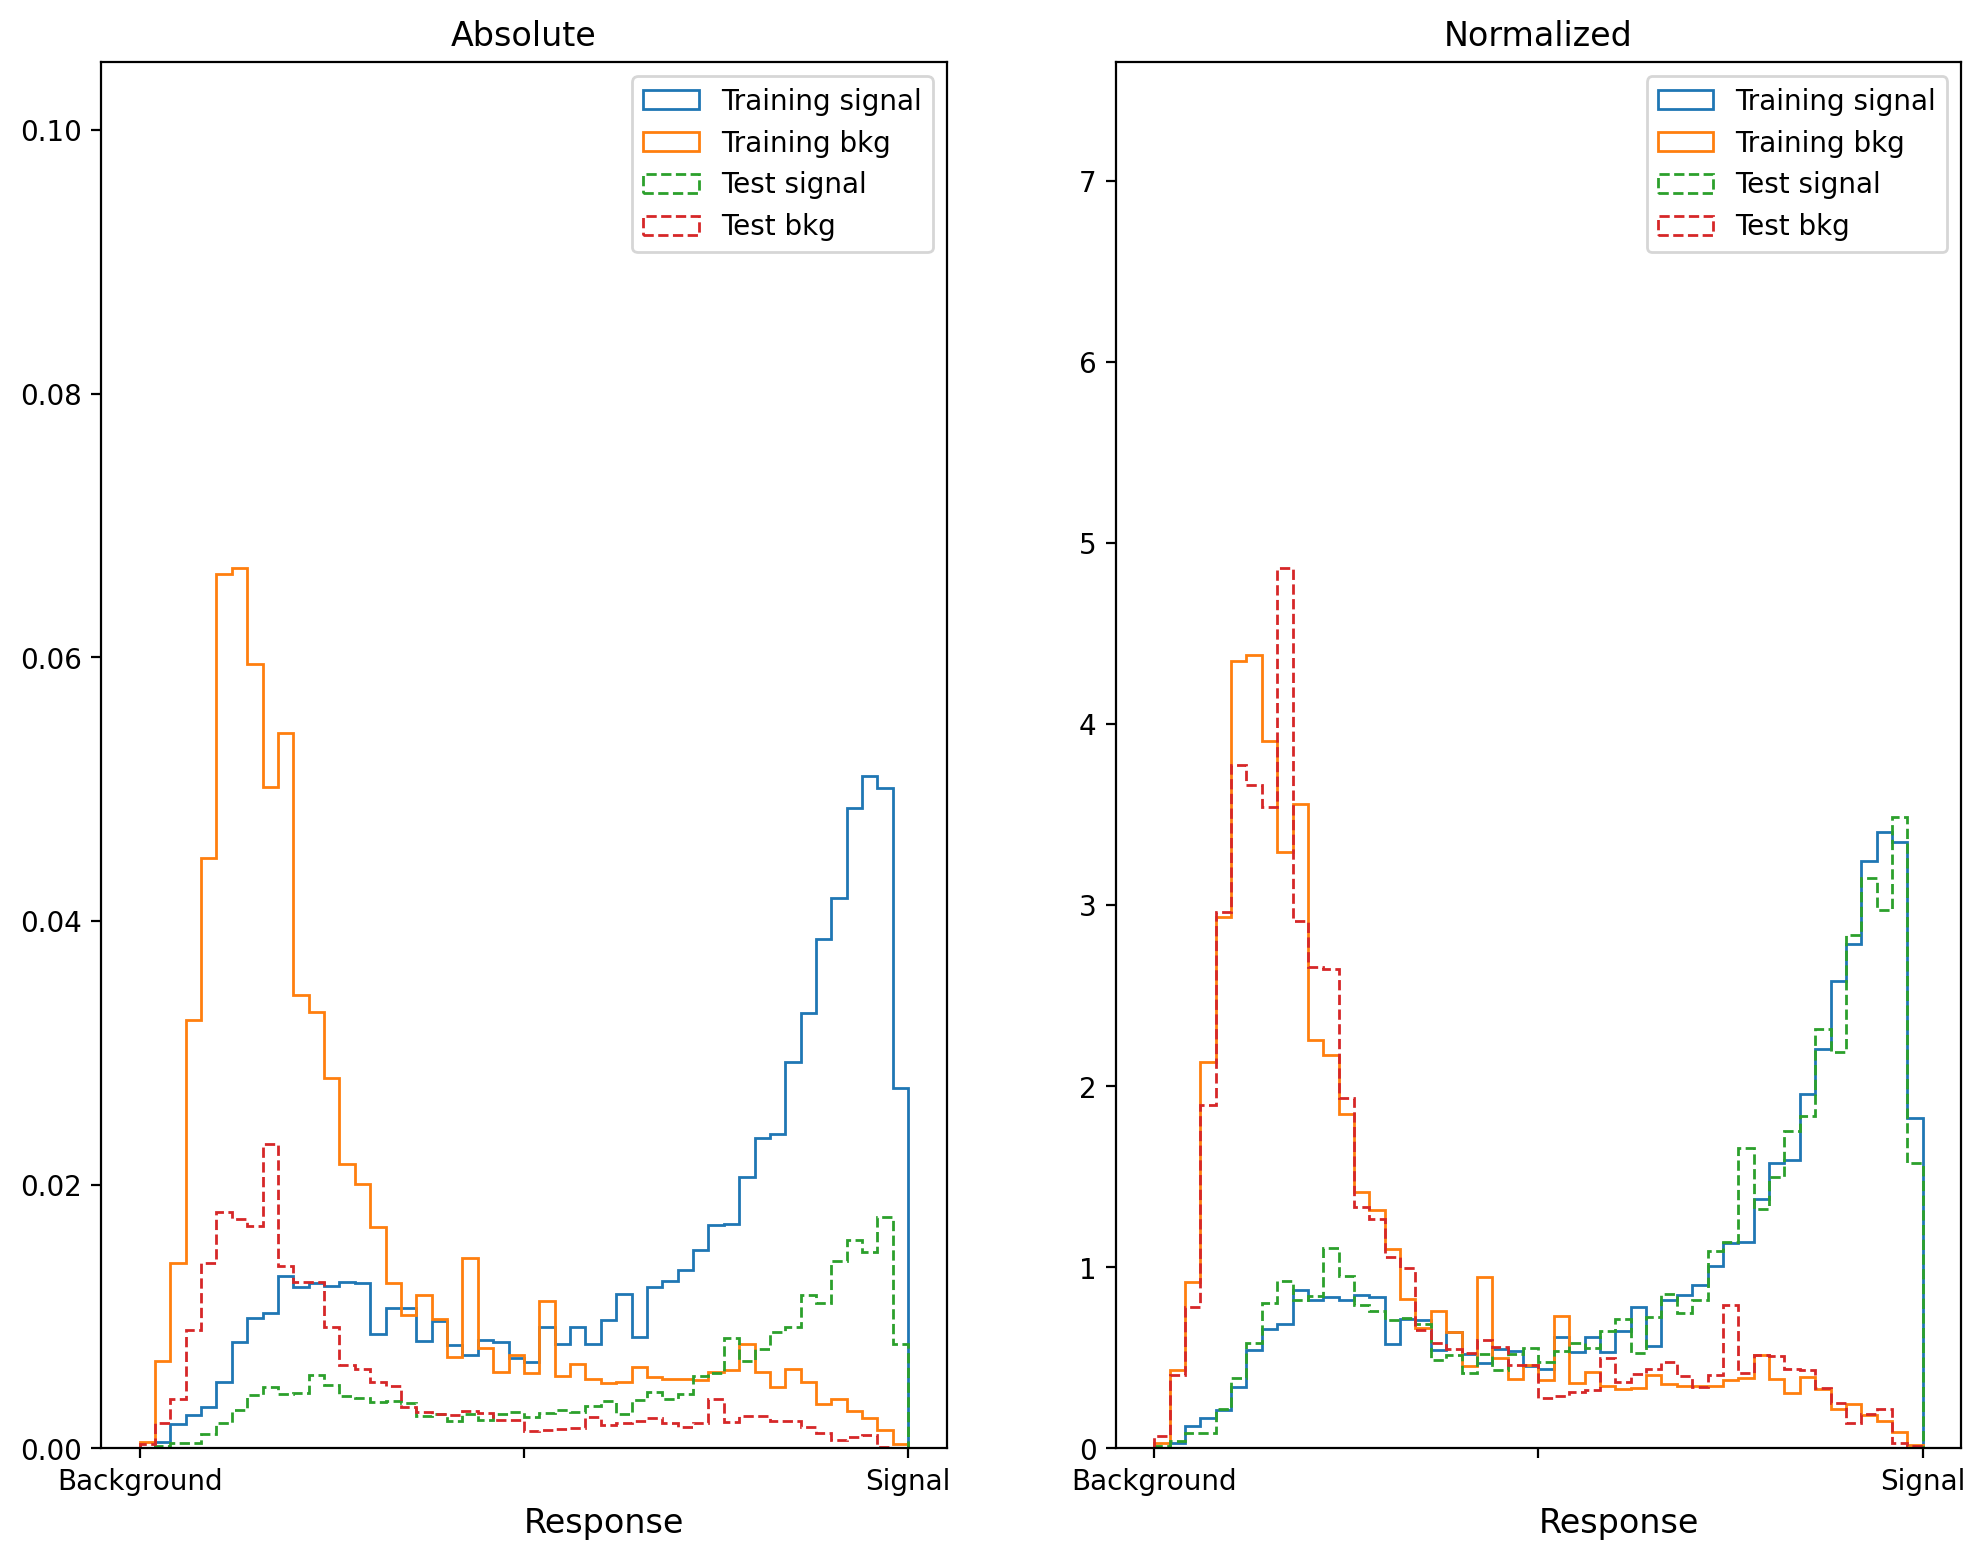
\includegraphics[width=\textwidth]{response.png}
    \end{figure}
  \end{column}
  \begin{column}{0.5\textwidth}
    \begin{figure}
      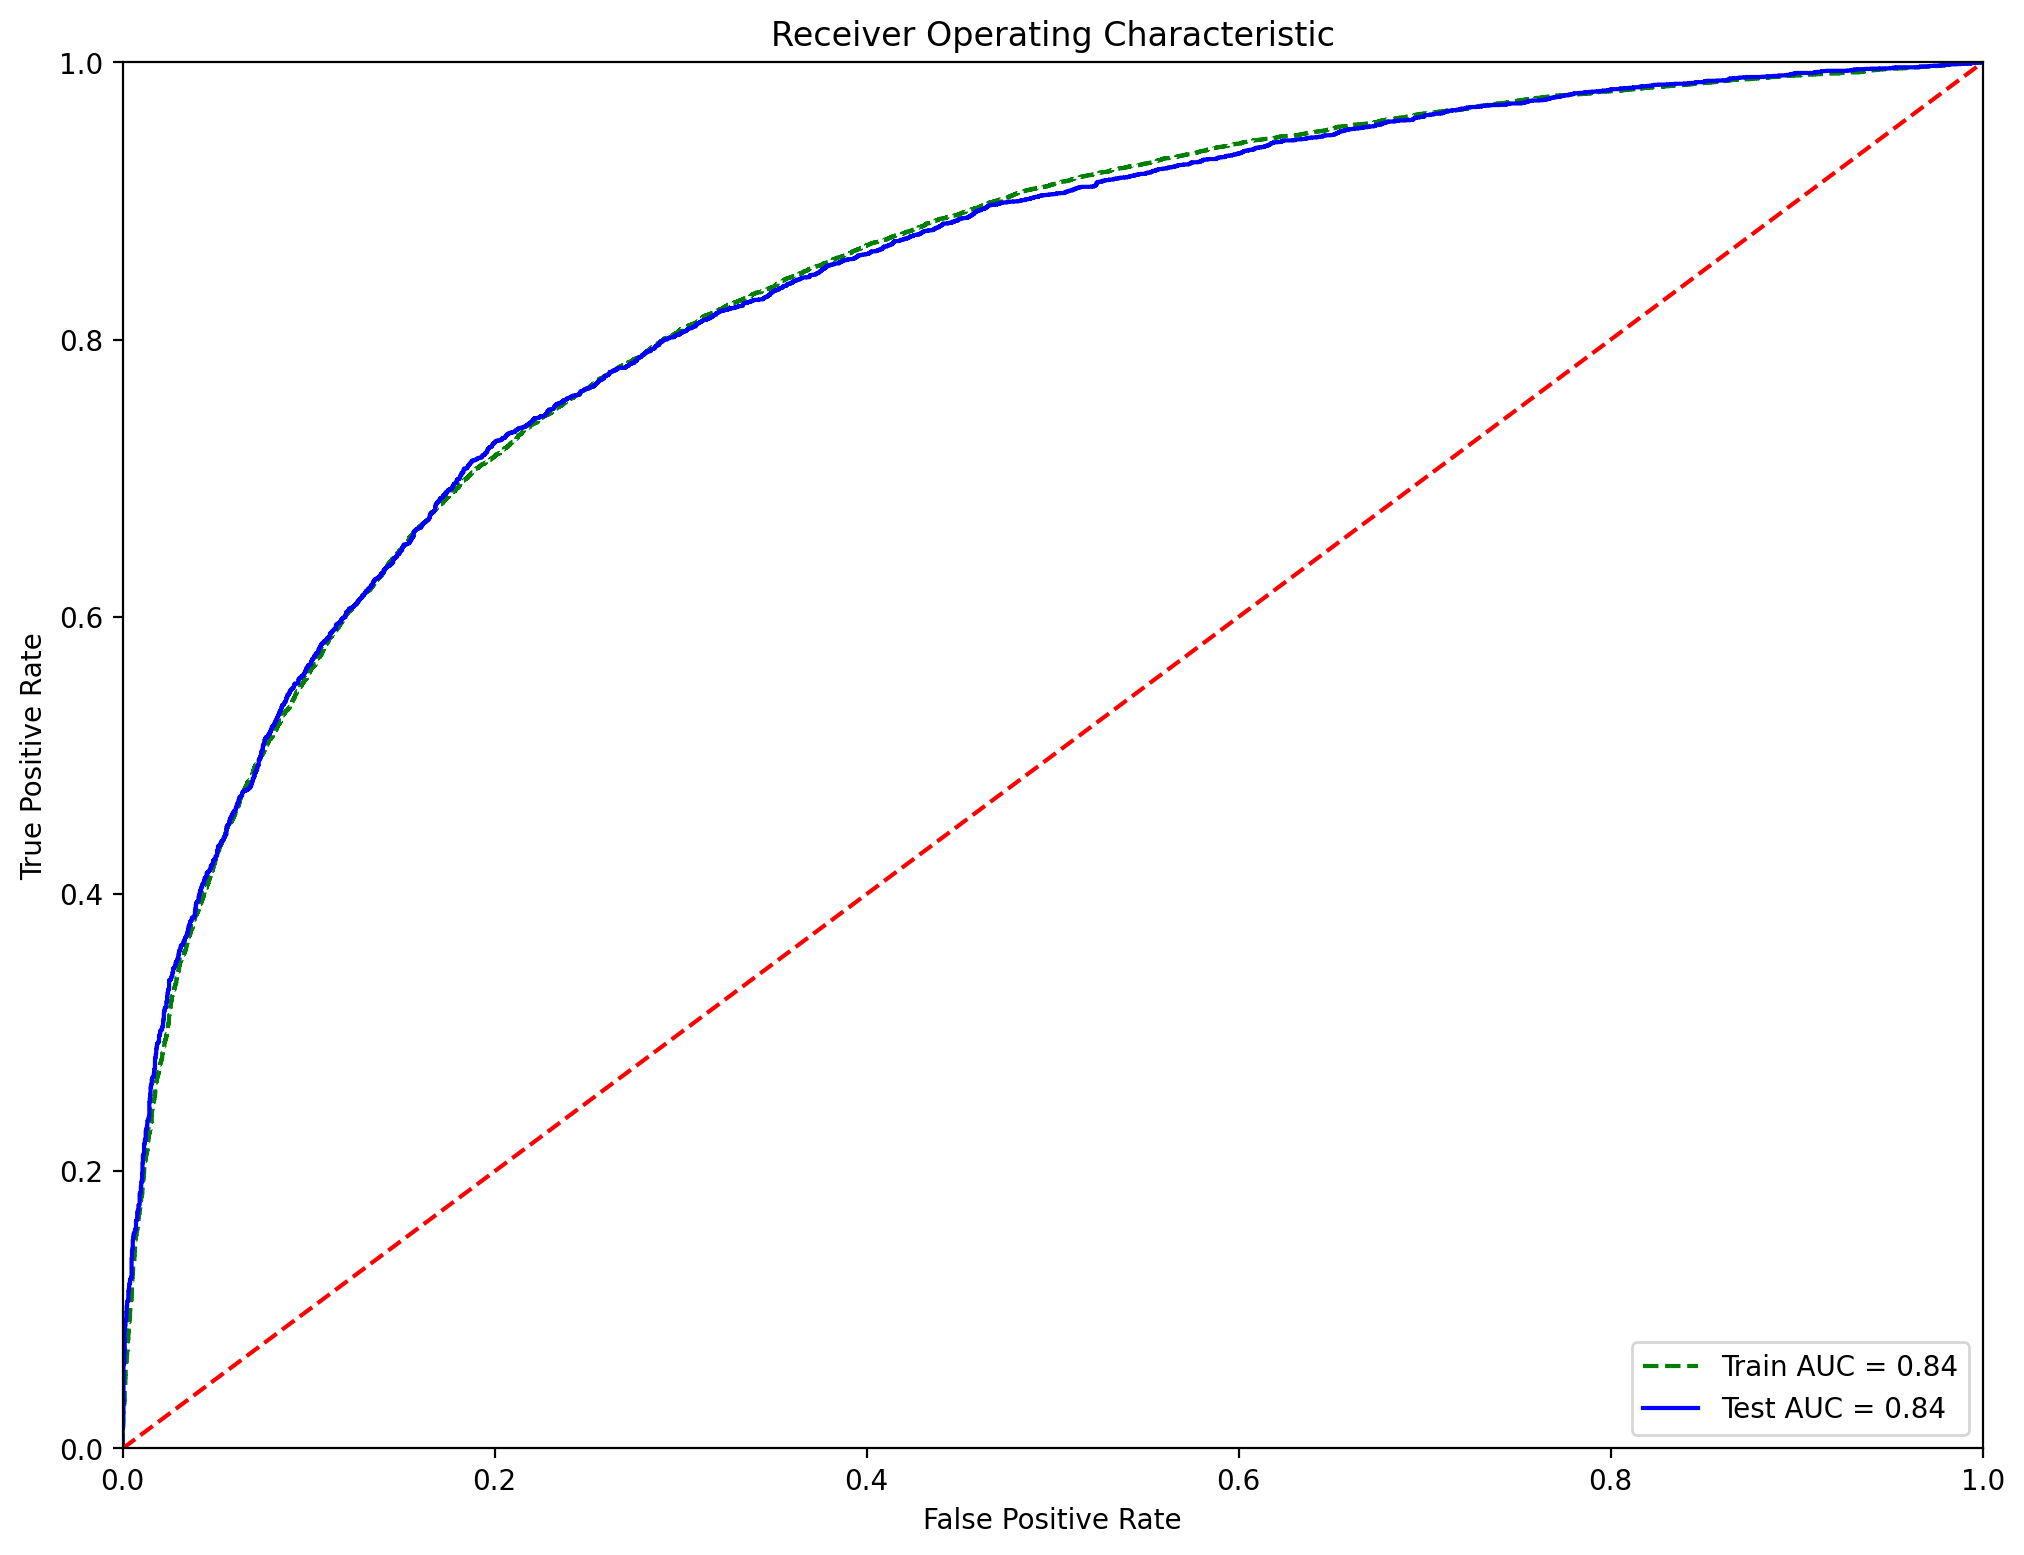
\includegraphics[width=\textwidth]{ROC.png}
    \end{figure}
  \end{column}
\end{columns}
%
\begin{itemize}
  \item Really good separation for this early stage of Optimisation
  \item Slight problems in training and validation agreement
\end{itemize}
\end{frame}


\begin{frame}{Lorentz invariant variables}
  \begin{columns}
    \begin{column}{0.5\textwidth}
      \begin{itemize}
        \item ip\_l1l2
        \item ip\_l1l3
        \item ip\_l2l3
        \item ip\_l1j1
        \item ip\_l1j2
        \item ip\_l1j3
        \item ip\_l1j4
        \item ip\_l1j5
        \item ip\_l2j1
        \item ip\_l2j2
        \item ip\_l3j1
        \item ip\_l3j2
      \end{itemize}
    \end{column}
    \begin{column}{0.5\textwidth}
      \begin{itemize}
        \item ip\_j1j2
        \item ip\_hadhad
        \item ip\_had1lep
        \item ip\_had2lep
        \item ip\_had1b
        \item ip\_had2b
        \item ip\_lepb
        \item ip\_had1jf
        \item ip\_had2jf
        \item ip\_lepjf
        \item ip\_bjf
        \item m\_met
      \end{itemize}
    \end{column}
  \end{columns}
\end{frame}

\begin{frame}
    \begin{table}[]
    \begin{tabular}{|l|l|}
    \hline
    Hyperparameter          & Setting             \\ \hline
    Nodes                   & 240                 \\ \hline
    Layers                  & 2                   \\ \hline
    Dropout                 & 0.9                 \\ \hline
    Batchnormalisation       & On                  \\ \hline
    Activation              & elu                 \\ \hline
    Output activation       & sigmoid             \\ \hline
    Batch size              & 1000                \\ \hline
    Optimisation            & Adam                \\ \hline
    Weight Initialisation   & Lecun Normalisation \\ \hline
    \end{tabular}
    \end{table}
\end{frame}

\begin{frame}{Results}
\begin{columns}
  \begin{column}{0.5\textwidth}
    \begin{figure}
      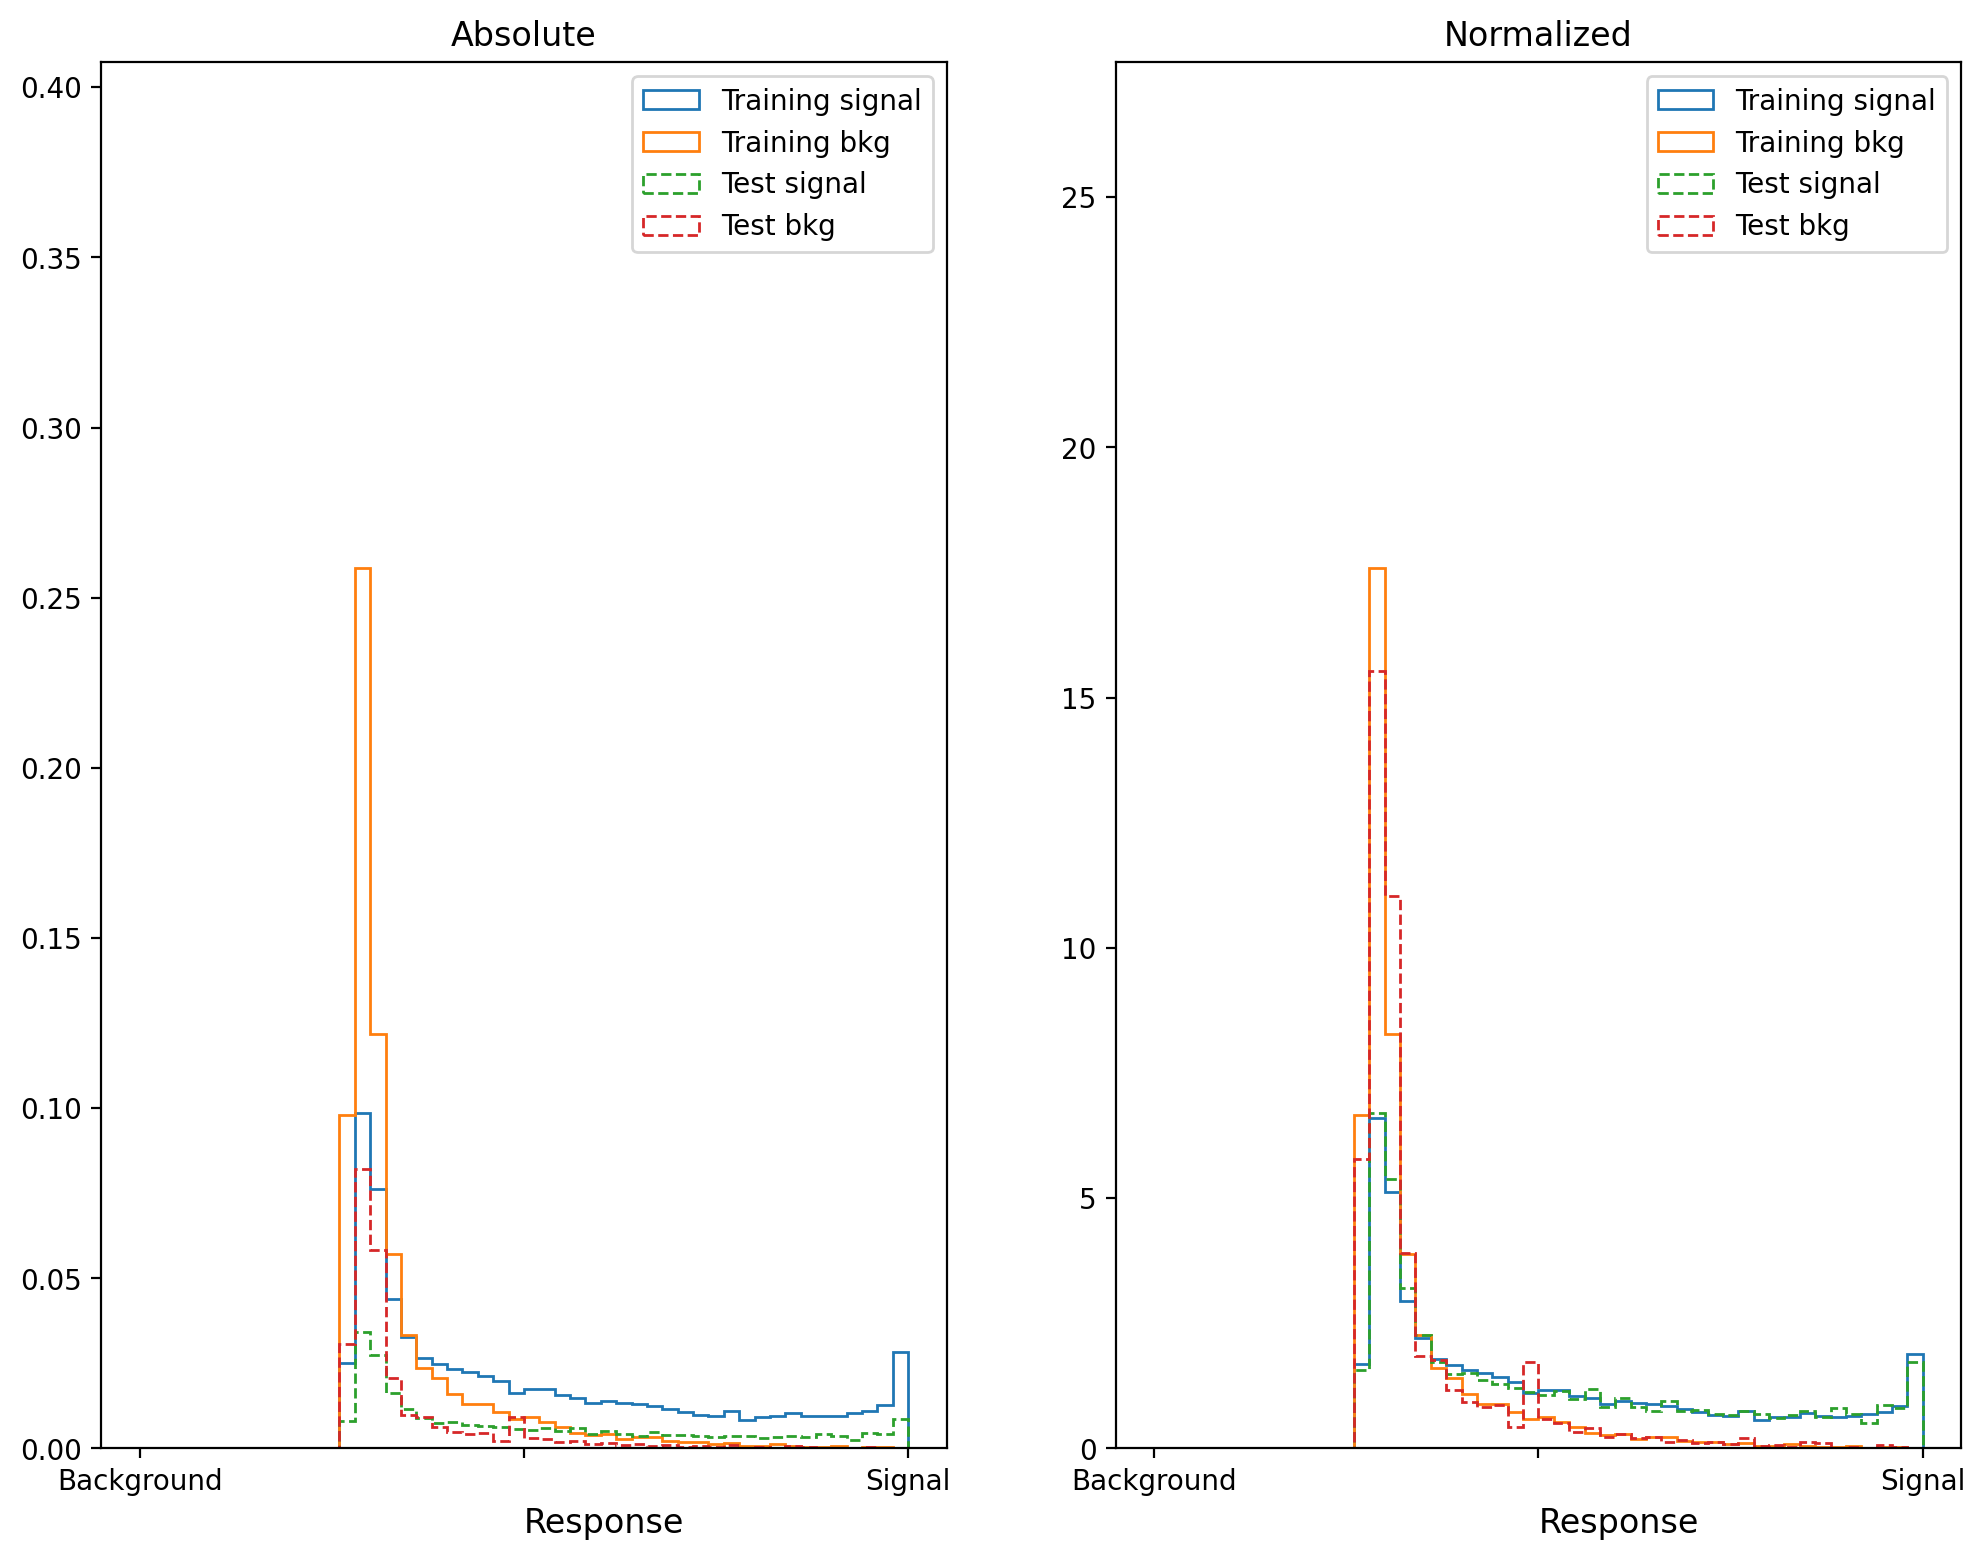
\includegraphics[width=\textwidth]{Response_Lorentz}
    \end{figure}
  \end{column}
  \begin{column}{0.5\textwidth}
    \begin{figure}
      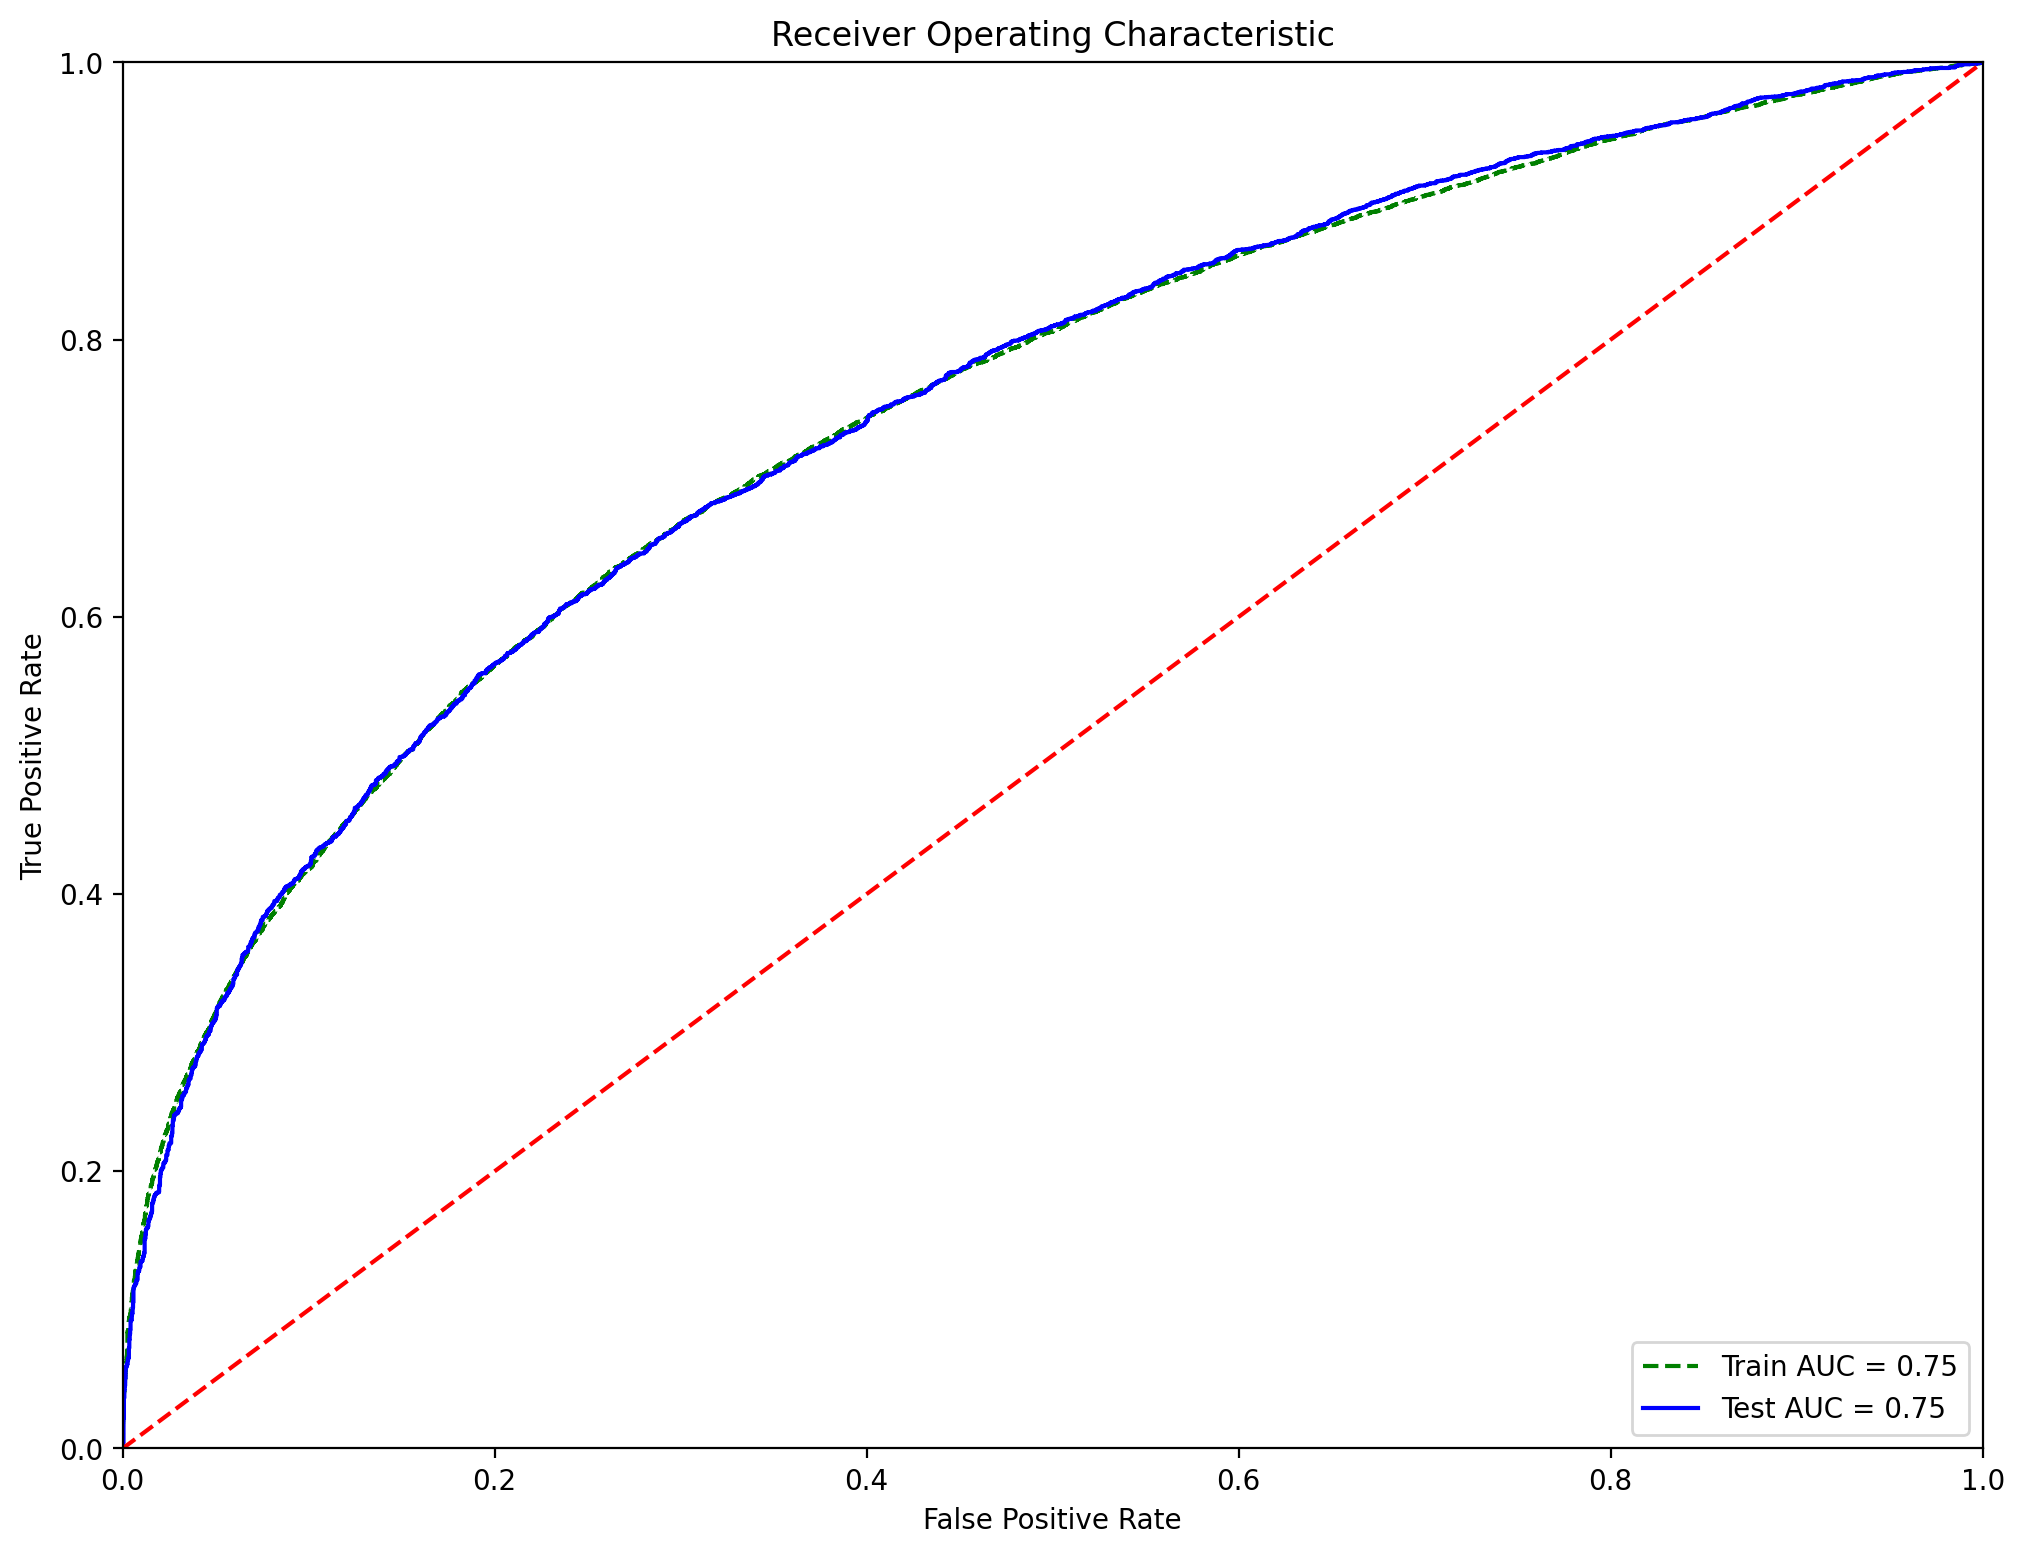
\includegraphics[width=\textwidth]{ROC_Lorentz}
    \end{figure}
  \end{column}
\end{columns}
%
\begin{itemize}
  \item Bad separation
  \item Only good point is the stability
\end{itemize}
\end{frame}